\RequirePackage{amsmath}
\documentclass[twocolumn, times]{aastex63}
\usepackage[spanish,es-minimal,english]{babel}
\usepackage[utf8]{inputenc}
\usepackage{natbib}
%\usepackage{microtype}
\usepackage{hyperref}
\usepackage{savesym}
\savesymbol{tablenum}
\usepackage{siunitx}
\restoresymbol{SIX}{tablenum}
\usepackage[varg]{newtxmath}
\usepackage{newtxtext}
\usepackage{booktabs}
\usepackage{array}   % for \newcolumntype macro
\newcolumntype{L}{>{$}l<{$}} % math-mode version of lrc column types
\newcolumntype{R}{>{$}r<{$}} 
\newcolumntype{C}{>{$}c<{$}} 

\bibliographystyle{aasjournal}

\newcommand\ION[2]{#1\,\scalebox{0.9}[0.8]{\uppercase{#2}}}
\newcounter{ionstage}
\renewcommand{\ion}[2]{\setcounter{ionstage}{#2}% 
  \ensuremath{\mathrm{#1\,\scriptstyle\Roman{ionstage}}}}
\newcommand\hii{\ion{H}{2}}
\newcommand\Raman{\ensuremath{_{\text{Raman}}}}
\def\th#1#2{\(\theta^{#1}\)\,Ori~#2}
\newcommand\wn{\ensuremath{\tilde{\nu}}}

% Chemical formulae
\newcommand*\chem[1]{\ensuremath{\mathrm{#1}}}
% Atomic term symbols
\newcommand\Config[1]{\ensuremath{\mathrm{#1}}}
\newcommand\Term[3]{\ensuremath{\mathrm{#1\ ^{#2}#3}}}
\newcommand\Level[4]{\ensuremath{\mathrm{#1\ ^{#2}#3_{#4}}}}

\newcommand\ha{\ensuremath{\text{H}\alpha}}
\newcommand\lya{\ensuremath{\text{Ly}\alpha}}
\newcommand\lyb{\ensuremath{\text{Ly}\beta}}

\begin{document}
\title{Extinction and scattering of nebular emission in Orion}
\shorttitle{Extinction anomalies in the Orion Nebula}
\author{William J. Henney}
\affiliation{%
  \foreignlanguage{spanish}{Instituto de Radioastronomía y
    Astrofísica, Universidad Nacional Autónoma de México, Apartado
    Postal 3-72, 58090 Morelia, Michaoacán, Mexico}}
\email{w.henney@irya.unam.mx}

\begin{abstract}
  I compare several different methods for estimating the dust
  extinction of diffuse emission from \hii{} regions.  Using archival
  data for the Orion Nebula, I show that apparent discrepancies
  between the different methods are powerful diagnostics of
  (1)~emission line scattering from dusty PDRs; (2)~the presence of
  dust layers sandwiched between two emitting gas layers; and (3)~the
  presence of deeply embedded ionized gas that is invisible at optical
  and near-infrared wavelengths.
\end{abstract}

\keywords{Atomic physics; Radiative transfer; Photodissociation regions}
\facilities{VLT:Yepun (MUSE); VLA}
%\object{M42}

\section{Introduction}
\label{sec:introduction}

\begin{figure}
  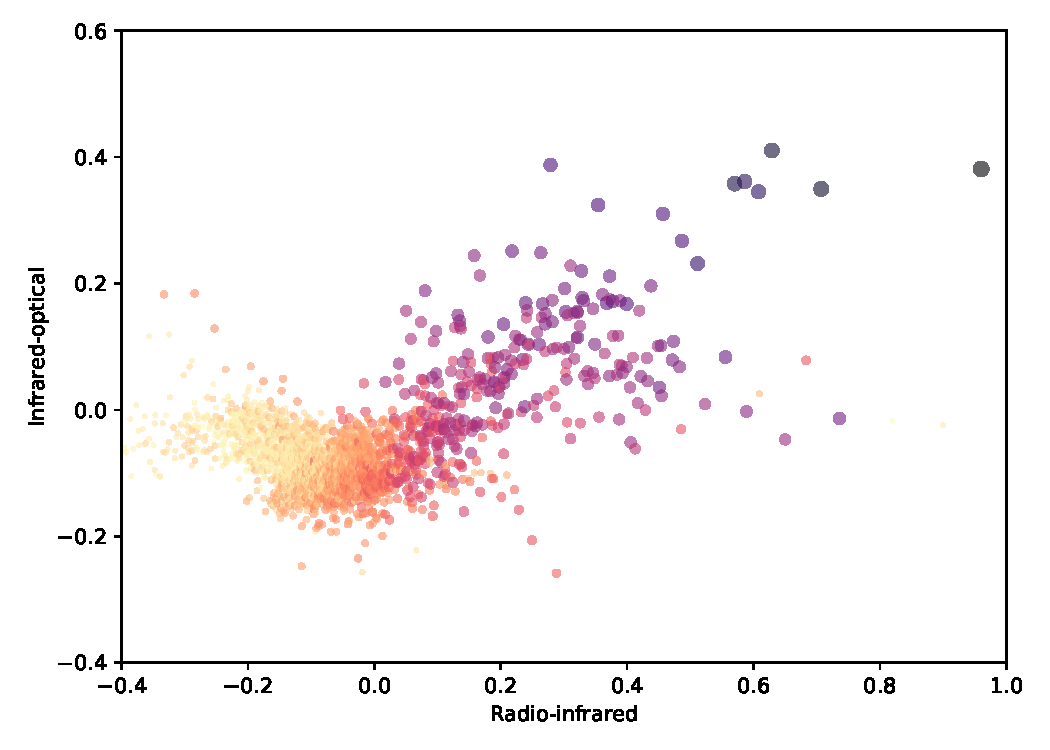
\includegraphics[width=\linewidth]{figs/orion-extinction-anomalies-scatter-bin032}
  \caption{Scatter plot of the infrared/optical extinction anomaly
    versus the radio/infrared extinction anomaly.  Plot symbol color
    and size indicate the optical--radio extinction (larger values are
    darker and larger).}
\end{figure}

\begin{figure*}
  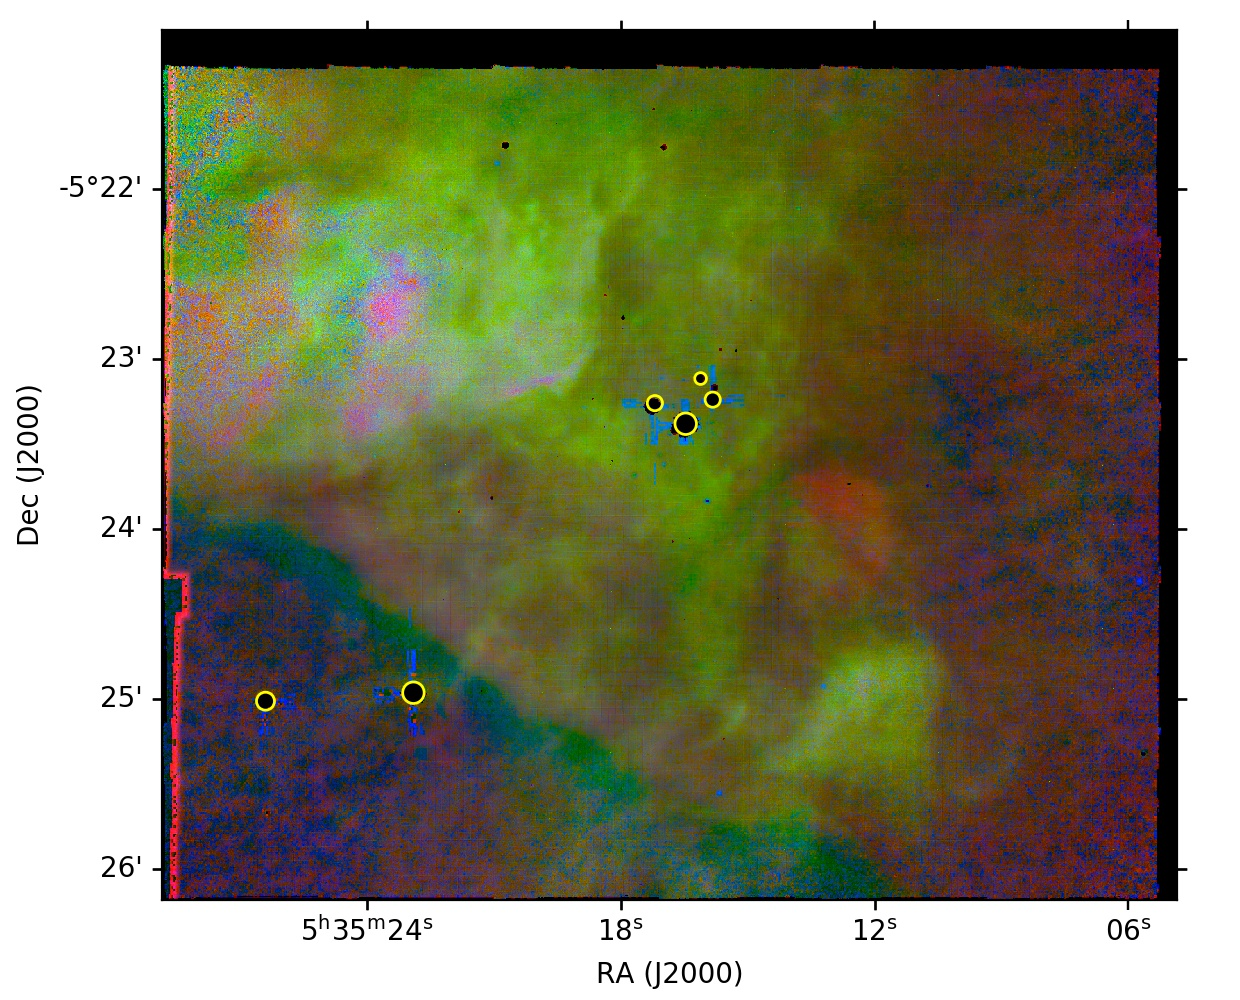
\includegraphics[width=\linewidth]{figs/rgb-lupton-extinction}
  \caption{Three-color image of extinction in the inner Orion
    Nebula. Extinction derived from the optical band reddening of the
    Balmer decrement (\SIrange{4886}{6563}{\angstrom}) is shown in
    green.  The infrared/optical extinction anomaly is shown in blue
    and the radio/infrared extinction anomaly is shown in red.}
  \label{fig:3color-extinction}
\end{figure*}

\section{Other measures of extinction}
\label{sec:other-meas-extinct}

\subsection{Diffuse interstellar bands}
\label{sec:diff-interst-bands}

\SI{5781}{\angstrom} is the cleanest.
There is also \SI{6283}{\angstrom},
which is stronger,
but it is affected by the telluric \chem{O_2} absorption.


\subsection{Forbidden metal doublets}
\label{sec:forb-metal-doubl}

We can use two lines that share an upper level.
Small wavelength range, but high S/N and rock-solid intrinsic ratio.

[\ion{O}{3}] \num{4959} and \SI{5007}{\angstrom} is a 1\% change in wavelength.  We see about a 1\% variation in the ratio.

[\ion{Ar}{3}] \num{7751} and \SI{7136}{\angstrom} is a 9\% change in wavelength.  We see about a 15\% variation in the ratio.  We also see scattering in the Bar PDR (reduction in reddening).

These give the gradient, \( d A_\lambda / d \lambda\)

\subsection{Continuum colors}
\label{sec:continuum-colors}

Broad band colors of the pure continuum can be a diagnostic of scattered light.

We should try and subtract off the atomic continuum. 



\bibliography{BibdeskLibrary}

\end{document}
%%% Local Variables:
%%% mode: latex
%%% TeX-master: t
%%% End:
